% =====================================================================
% Clase -- Geometría 8° -- Trimestre I -- Semana 04
% Sesión 004 (mar 22 sep., 11:00, 50 min)
% Tema: Congruencia de triángulos
% Subtema: Criterios de congruencia: LLL, LAL, ALA
% Hilo conductor del trimestre I: «Tales de Mileto y la medición de la gran pirámide»
% Tema 2 de la guía: Congruencia de triángulos (tema:congruencia)
% Material del docente (no se entrega a los estudiantes).
% =====================================================================
\documentclass[11pt]{article}
\makeatletter\def\input@path{{../../../../../plantillas/estilo/}}\makeatother
\usepackage{mmcantillo}
\guiadelestudiante{../../guia-didactica/guia-periodo-I-triangulos}

\tipodocumento{Clase}
\asignatura{Geometría}
\titulo{Semana 4: el barco de Tales}
\grado{8°}
\periodo{I}

% DBA: matematicas grado 8 · DBA 6 — Identifica relaciones de congruencia y semejanza
% entre las formas geométricas que configuran el diseño de un objeto. Evidencias de esta
% sesión: «Utiliza criterios para argumentar la congruencia de dos triángulos» y «Compara
% figuras y argumenta la posibilidad de ser congruente o semejantes entre sí».

\begin{document}

\encabezado*

\begin{center}
{\renewcommand{\arraystretch}{1.3}
\begin{tabularx}{\linewidth}{@{}l l l X l@{}}
  \toprule
  \textbf{Sesión} & \textbf{Fecha} & \textbf{Min} & \textbf{Subtema} & \textbf{Entregables}\\
  \midrule
  004 & mar 22 sep., 11:00 & 50 & Criterios de congruencia: LLL, LAL, ALA
      & Taller; se recoge la tarea\\
  \bottomrule
\end{tabularx}}
\end{center}

Segundo paso del hilo: según Eudemo, Tales calculaba desde la costa la distancia a un barco.
La clase muestra por qué eso es posible: tres datos bien escogidos determinan un triángulo,
y un triángulo determinado se puede copiar en tierra firme.
Referencia: \refguia{tema:congruencia}.

% ---------------------------------------------------------------------
\seccion{Sesión 004 — martes 22 de septiembre · 11:00 · 50 min}

\textbf{Objetivo.} Reconocer cuándo dos triángulos son congruentes y justificarlo con el
criterio adecuado (LLL, LAL o ALA), explicando por qué tres ángulos iguales no bastan.

\textbf{Materiales.} Tablero; tres pitillos o palitos de longitudes distintas y cuatro de
igual longitud con plastilina o chinches; regla, transportador y compás; la guía.

\begin{center}
{\renewcommand{\arraystretch}{1.3}
\begin{tabularx}{\linewidth}{@{}l l X@{}}
  \toprule
  \textbf{Momento} & \textbf{Min} & \textbf{Actividad}\\
  \midrule
  Tarea & 0--5 & Recoger la tarea. Resolver en voz alta solo la del ángulo recto (pregunta
    3) como puente: «¿cuántos datos necesitamos para saber todo de un triángulo?»\\
  Enganche & 5--10 & Armar con pitillos un triángulo y un cuadrilátero y empujarlos: el
    cuadrilátero se aplasta y el triángulo no. Con tres longitudes fijas solo sale
    \emph{un} triángulo (aplicación de la guía: torres, puentes, cerchas).\\
  Explicación & 10--22 & Definición de congruencia y notación $\triangle ABC \cong
    \triangle DEF$ (el orden de las letras indica la correspondencia). Criterios LLL, LAL,
    ALA, con dibujo en el tablero marcando lados y ángulos iguales con rayitas y arcos.
    Subrayar la palabra \emph{comprendido}. Contraejemplo de AAA: un triángulo y su
    ampliación ($3$-$4$-$5$ y $6$-$8$-$10$) — se retoma en semejanza.\\
  El barco de Tales & 22--27 & Leer el ejemplo de la guía. Pregunta: «¿qué tres datos mide
    Tales y cuál criterio usa?» (el lado $AB$ y los dos ángulos de sus extremos: ALA).\\
  Taller & 27--47 & Taller individual (5 puntos). La pregunta 2 requiere regla y
    transportador; quien no tenga transportador, trabaja en pareja.\\
  Cierre & 47--50 & Recoger el taller. Anuncio: la próxima semana, construir triángulos
    congruentes con regla y compás.\\
  \bottomrule
\end{tabularx}}
\end{center}

\textbf{Figura para el tablero: los tres criterios.}

\begin{center}
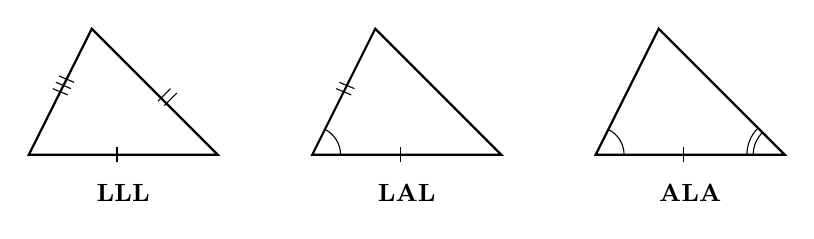
\begin{tikzpicture}[scale=0.8, every node/.style={font=\small}]
  % LLL
  \begin{scope}
    \draw[thick] (0,0) -- (3,0) -- (1,2) -- cycle;
    \draw (1.4,-0.12) -- (1.4,0.12);
    \draw (2.05,0.85) -- (2.25,1.05); \draw (2.15,0.78) -- (2.35,0.98);
    \draw (0.38,1.05) -- (0.62,0.95); \draw (0.43,1.15) -- (0.67,1.05);
    \draw (0.48,1.25) -- (0.72,1.15);
    \node at (1.5,-0.6) {\textbf{LLL}};
  \end{scope}
  % LAL
  \begin{scope}[xshift=4.5cm]
    \draw[thick] (0,0) -- (3,0) -- (1,2) -- cycle;
    \draw (1.4,-0.12) -- (1.4,0.12);
    \draw (0.38,1.05) -- (0.62,0.95); \draw (0.43,1.15) -- (0.67,1.05);
    \draw (0.45,0) arc (0:63.4:0.45);
    \node at (1.5,-0.6) {\textbf{LAL}};
  \end{scope}
  % ALA
  \begin{scope}[xshift=9cm]
    \draw[thick] (0,0) -- (3,0) -- (1,2) -- cycle;
    \draw (1.4,-0.12) -- (1.4,0.12);
    \draw (0.45,0) arc (0:63.4:0.45);
    \draw (2.5,0) arc (180:135:0.5); \draw (2.4,0) arc (180:135:0.6);
    \node at (1.5,-0.6) {\textbf{ALA}};
  \end{scope}
\end{tikzpicture}

{\small Rayitas: lados iguales en los dos triángulos; arcos: ángulos iguales.}
\end{center}

\begin{nota}
El módulo de Geometría de \texttt{recursos/} da como primer criterio «dos ángulos iguales
$\Rightarrow$ congruentes»: es \textbf{falso} (solo da semejanza). Si algún estudiante lo
trae de un libro o de internet, es buena ocasión para el contraejemplo del triángulo y su
fotocopia ampliada. Tampoco se enseña LLA: con dos lados y un ángulo no comprendido pueden
salir dos triángulos distintos (basta mencionarlo, como en la guía).
\end{nota}

\begin{nota}
Las dos preguntas de congruencia del Tema 2 de la guía son las mismas que las preguntas 1 y
2 del taller (el banco no tiene más ejercicios de congruencia de 8°). Por eso, en esta
sesión no se trabajan en la guía antes del taller: la guía queda como material de estudio y
el taller es la primera vez que los estudiantes las resuelven.
\end{nota}

\end{document}
